\Cref{sec:photon_selection} introduced the best-photon candidate strategy, 
as well as selection to suppress events 
where the photon is misidentified or originates in sources different from \BtoXsgamma.
However, as was seen before in, for example, \Cref{fig:spectrum_after_reco},
\epem\ra\qqbar events provide the vast majority of photon candidates.
Therefore, a dedicated event selection for this type of background was devised.
It takes advantage of different event topologies expected for $\FourS\to\qqbar$ and $\epem\ra\qqbar$ events.
Events, where a $\FourS\to\BB$ decay is present, tend to be more `spherical' when compared with $\epem\ra\qqbar$ events exhibiting a `jet-like' distribution.
This is related to the fact that \epem collisions at $B$ factory experiments have just enough energy to produce a $B$ pair almost at rest, which means that its decays products, on average, tend to be distributed uniformly in polar and azimuthal angle.
On the other hand, light-quark pairs, produced in \epem collision events, also gain a substantial amount of back-to-back momentum which tends to spread their decay products. 
The schematic idea of this is shown in \Cref{fig:continuum_schematic}.
This section will provide an in-depth discussion on how the discrimination between \BtoXsgamma and continuum is achieved using a \BDT.

\begin{figure}[htbp!]
    \centering
    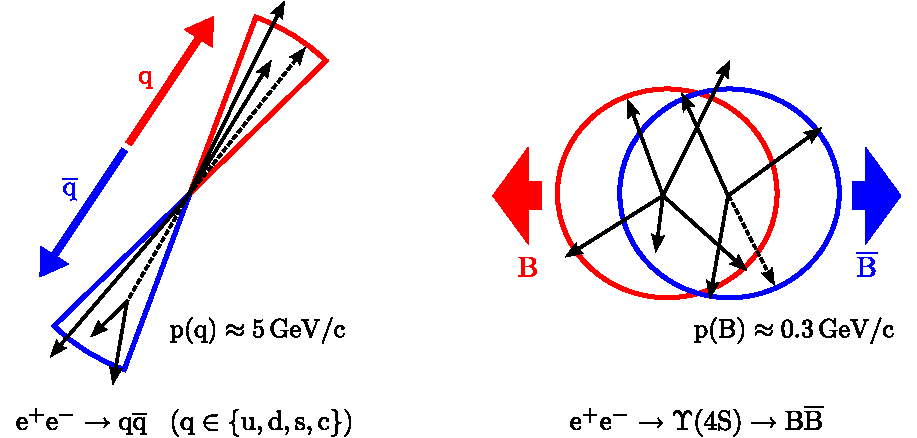
\includegraphics[width=0.6\textwidth]{figures/continuum_suppression/figure_continuum_suppression_event_shapes.pdf}
    \caption{\label{fig:continuum_schematic} Schematic illustration of continuum and \BB events created after an \epem collision in $B$ factories.
    Events, where a $B$ meson is produced, are generally more spherical since the \FourS is produced at rest and its decay products tend to not have a preferred direction.
    Typical momenta of light-quark and \BB mesons are shown.
    The specific directions shown are illustrative only. 
    }
\end{figure}

\subsection{Training event pre-selection}\label{sec:preselection}

Before a \BDT is trained, it is generally desirable to prepare the datasets such that the classifier 
learns based on relevant data.
Such data preprocessing will be performed based on variables described in \Cref{sec:photon_selection}.
The classifier will then be trained on the reduced dataset

In order to find optimal selections, a figure-of-merit study is performed for each observable.
Two figure-of-merit options were considered for this analysis, a more standard figure-of-merit $\mathrm{FOM}_1$:
\begin{equation}\label{eq:soversqrtsplusb}
    \mathrm{FOM}_1 = \frac{\mathsf{S}}{\sqrt{\mathsf{S}+\mathsf{B}}},
\end{equation}
and $\mathrm{FOM}_2$ defined in Ref.\cite{Punzi:2003bu} (often referred to as `Punzi' figure-of-merit):
\begin{equation}\label{eq:punzi_fom}
    \mathrm{FOM}_2 = \frac{\mathsf{S}}{\mathsf{S}_0} \frac{1}{\frac{3}{2}+\sqrt{\mathsf{B}}}.
\end{equation}
In both equations, $\mathsf{S}$ is the number of signal events after selection, 
$\mathsf{B}$ is the number of background events after selection, 
and $\mathsf{S}_0$ is the number of signal events before selection.
Although \Cref{eq:punzi_fom} was derived with search-like analyses in mind, 
it is utilised in this analysis to minimise signal model dependency: the ratio $\mathsf{S}/\mathsf{S}_0$ present in the definition reduces many model-dependant effects.

For each figure of merit calculation, background events ($\mathsf{B}$) are calculated based on generic \MC,
whereas signal events, $\mathsf{S}$, are calculated based on signal \MC, to ensure a high statistics sample.
In the case of \Cref{eq:soversqrtsplusb}, an appropriate scaling for $\mathsf{S}$ is also used.
Each dataset has duplicate tag-candidate events randomly removed, by picking a random tag-side candidate.
Each figure of merit is then calculated for 200 equally spaced selections in the target observable.
The maximum figure-of-merit point is taken as the optimal pre-selection for each of the variables.
This procedure is shown for $\mathrm{FOM}_2$ in \Cref{fig:selection_optimisations}.
Results for $\mathrm{FOM}_1$ are used as a cross-check for $\mathrm{FOM_2}$ but turn out to be consistent.
Equivalent procedure for $\mathrm{FOM}_1$ is shown in \Cref{sec:appendix_sqrtsplusb_optimisation}.
The resulting optimal selections are also shown in the Figures.

\begin{figure}[htbp!]
    \centering
    \subcaptionbox{\label{fig:bp_zmva_optimisation}}{
            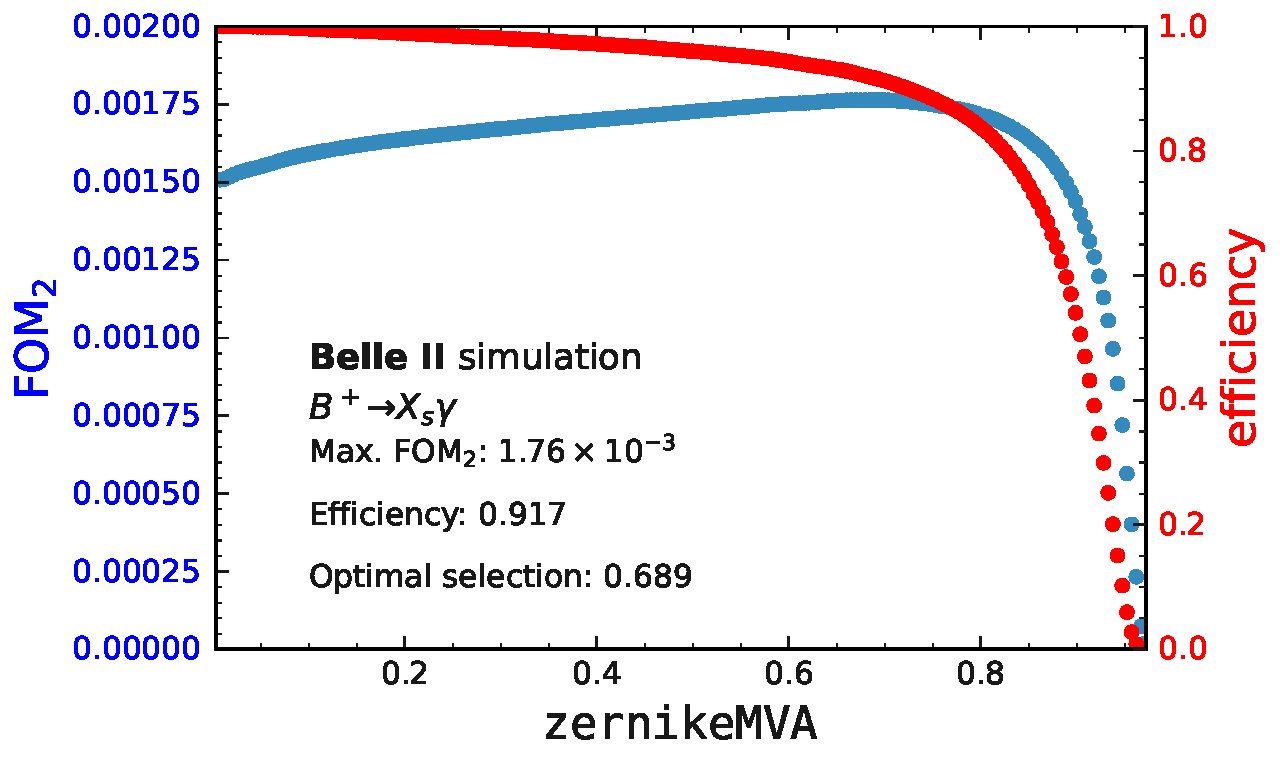
\includegraphics[width=0.3\textwidth]{figures/continuum_suppression/Bp_zernikeMVA_optimisation_punzi.pdf}
        }
    \subcaptionbox{\label{fig:bp_piveto_optimisation}}{
            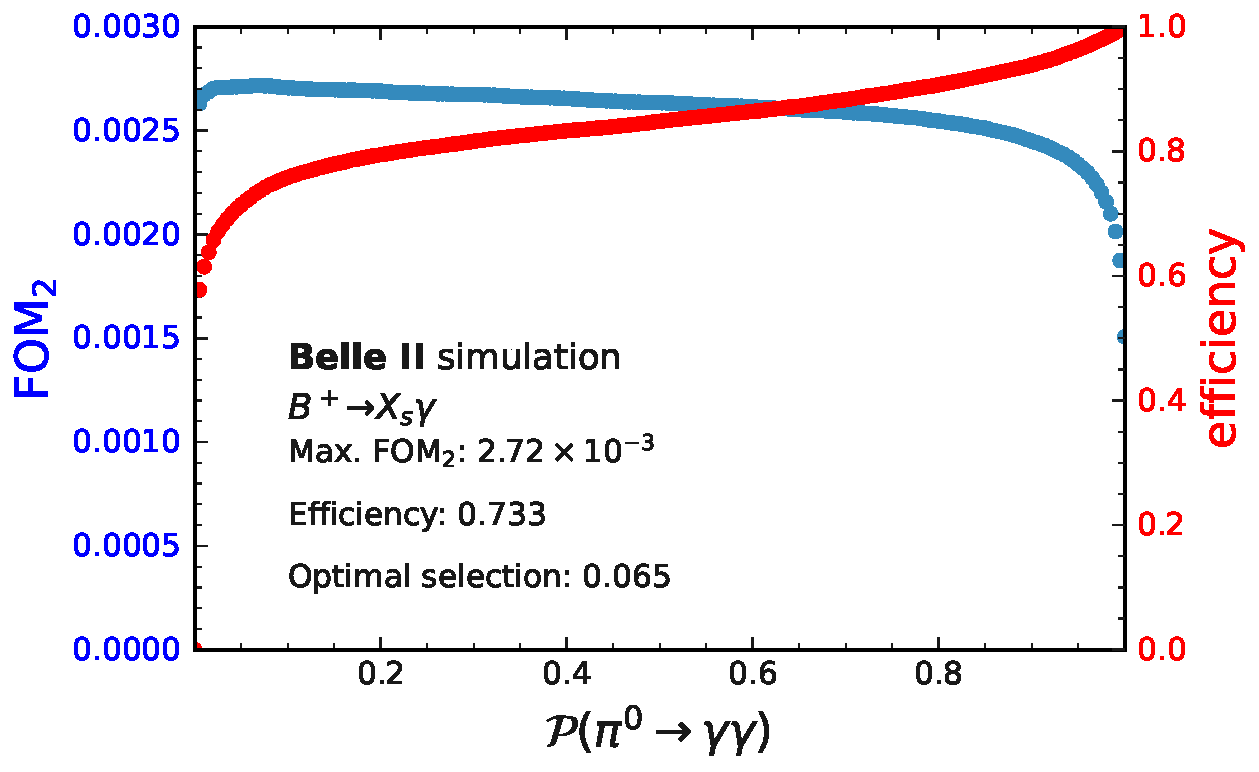
\includegraphics[width=0.3\textwidth]{figures/continuum_suppression/Bp_piVeto_optimisation_punzi.pdf}
        }
    \subcaptionbox{\label{fig:bp_etaveto_optimisation}}{
            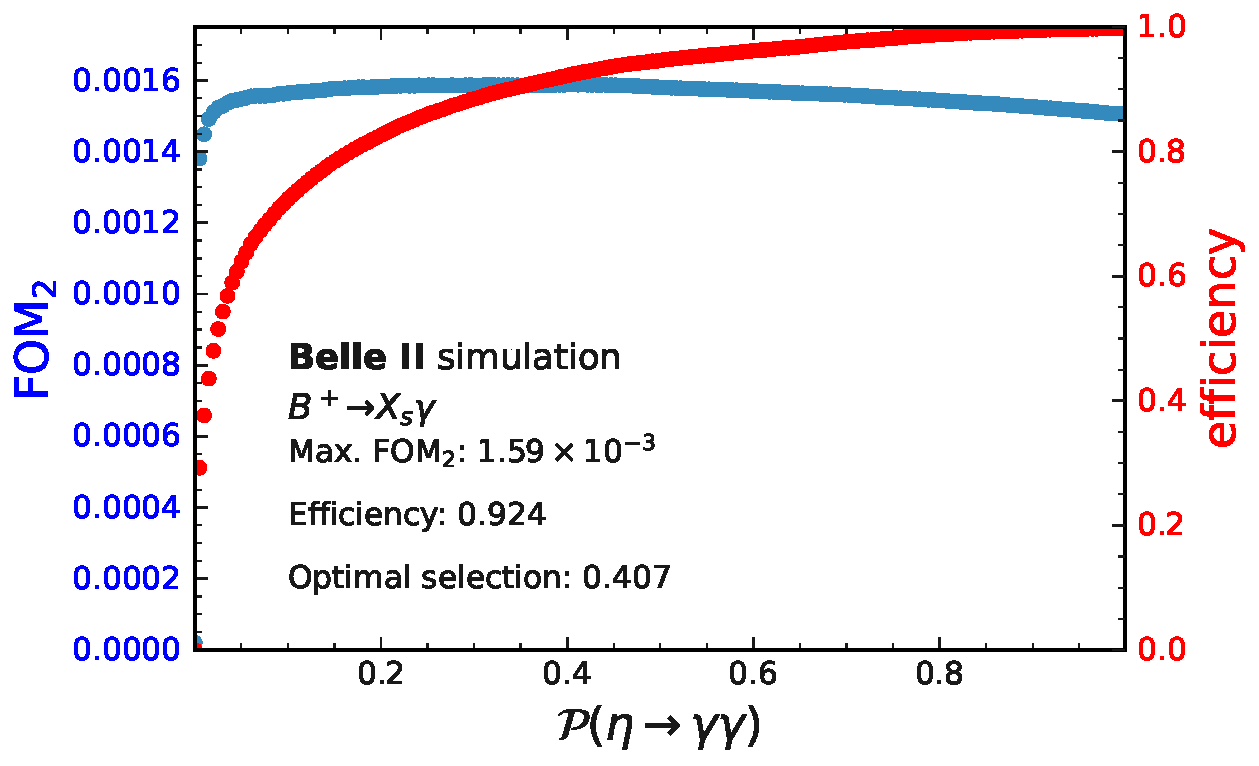
\includegraphics[width=0.3\textwidth]{figures/continuum_suppression/Bp_etaVeto_optimisation_punzi.pdf}
        }
    \subcaptionbox{\label{fig:bz_zmva_optimisation}}{
            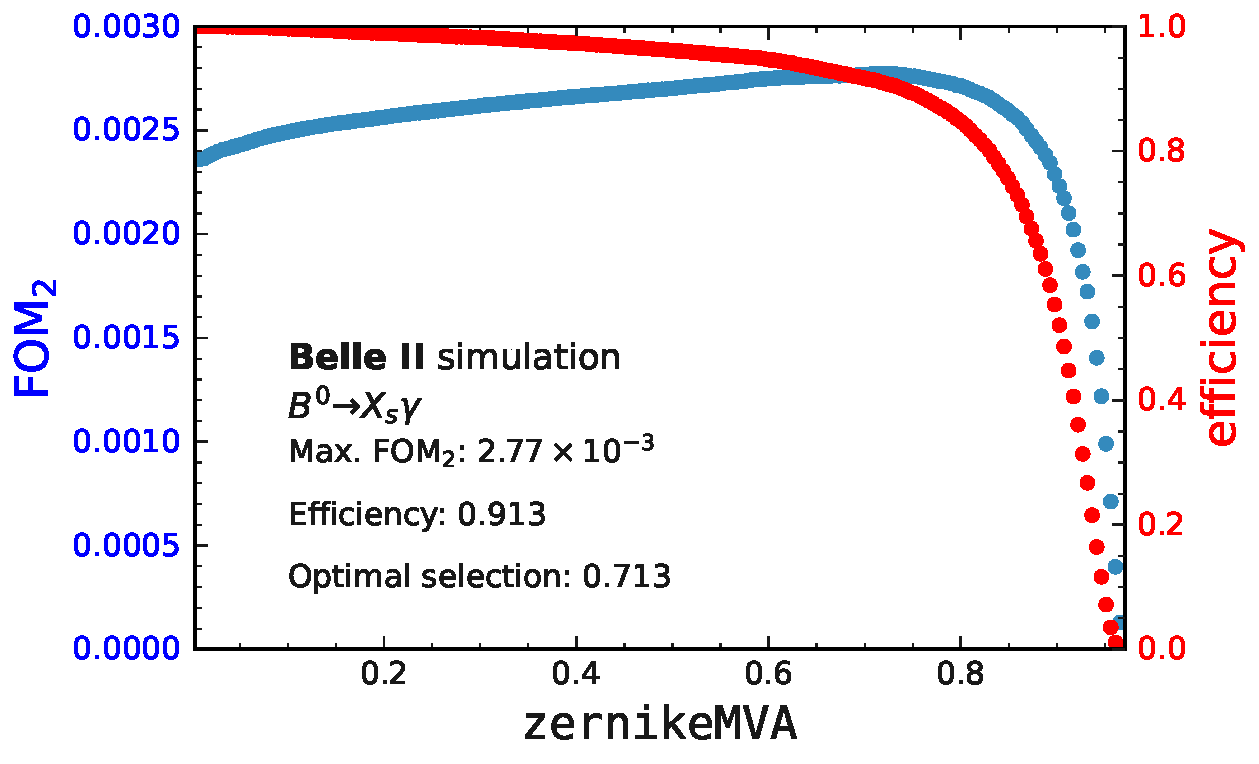
\includegraphics[width=0.3\textwidth]{figures/continuum_suppression/Bz_zernikeMVA_optimisation_punzi.pdf}
        }
    \subcaptionbox{\label{fig:bz_piveto_optimisation}}{
            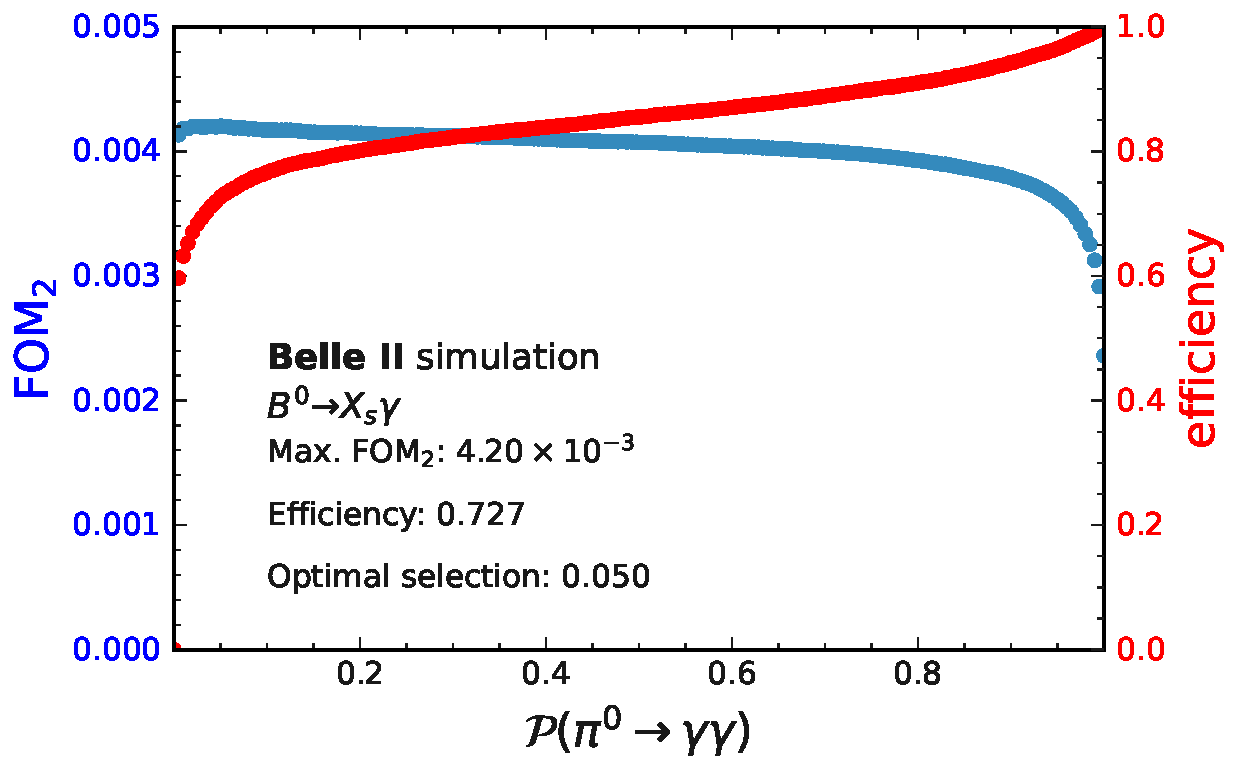
\includegraphics[width=0.3\textwidth]{figures/continuum_suppression/Bz_piVeto_optimisation_punzi.pdf}
        }
    \subcaptionbox{\label{fig:bz_etaveto_optimisation}}{
            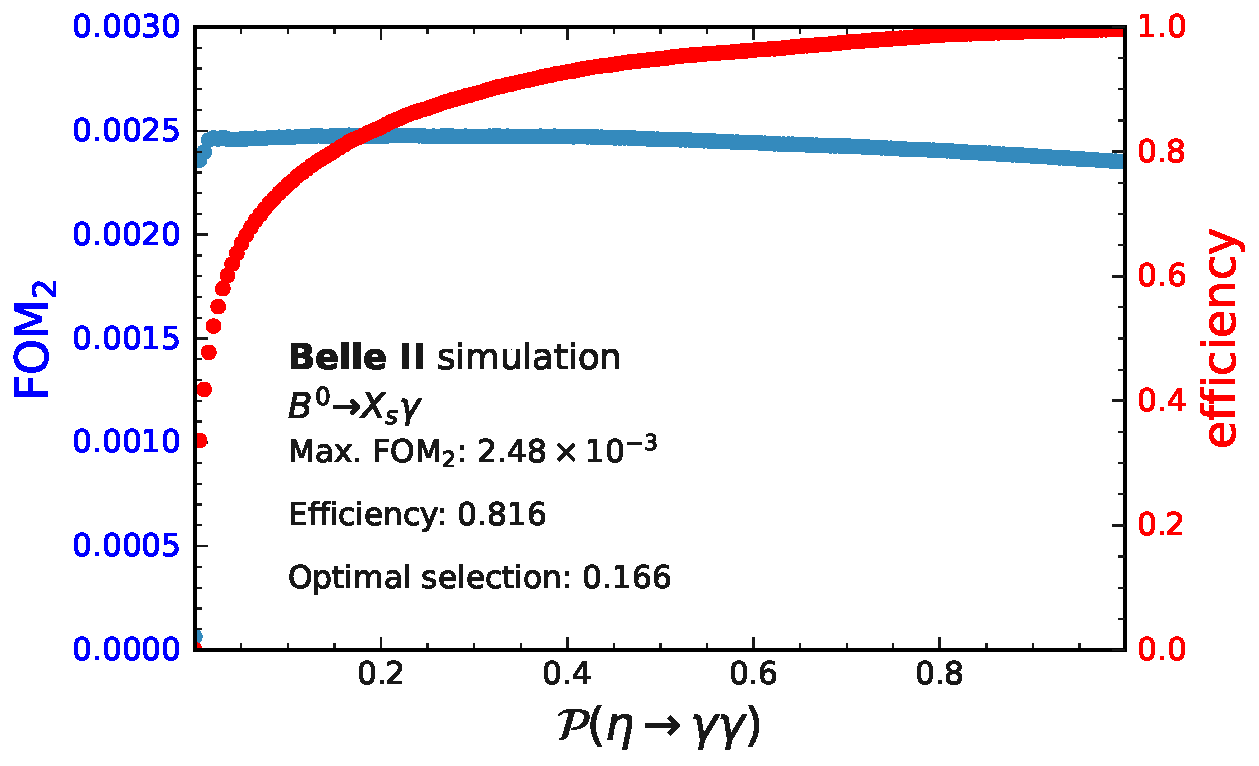
\includegraphics[width=0.3\textwidth]{figures/continuum_suppression/Bz_etaVeto_optimisation_punzi.pdf}
        }
    \caption{\label{fig:selection_optimisations} Optimal selection calculation for observables
    described in \Cref{sec:photon_selection} based on $\mathrm{FOM}_2$ (see \Cref{eq:punzi_fom}).
    For \BptoXsgamma events the tests are shown
    in \Cref{fig:bp_zmva_optimisation,fig:bp_piveto_optimisation,fig:bp_etaveto_optimisation},
    and for \BztoXsgamma in \Cref{fig:bz_zmva_optimisation,fig:bz_piveto_optimisation,fig:bz_etaveto_optimisation}.
    The figures show the efficiency and $\mathrm{FOM}_2$ score calculated for 200 selections of \piVeto, \etaVeto and \ZMVA.
    The maximum value of $\mathrm{FOM}_2$, the corresponding selection and efficiency are shown as well.
    }
\end{figure}

The results between \Bp and \Bz modes, as well as using $\mathrm{FOM}_1$ and $\mathrm{FOM}_2$ are consistent, with only marginal differences.
Therefore, due to the model independence of $\mathrm{FOM}_2$, this figure-of-merit will be the only one discussed henceforth.
At this stage, it is unnecessary to choose the `best' selection, 
as another simultaneous optimisation will be performed later, together with continuum suppression \BDT output in \Cref{sec:final_optimisation}.
The main goal is to reduce the sample size to include only relevant data, such that the trained \BDT can make decisions for difficult cases that are not easily distinguishable using simple selection.
Based on \Cref{fig:selection_optimisations}, pre-selections are chosen, which suppress background but retain most of the signal.
The requirements for a loose selection are tailored such that more roughly 75\% of \BtoXsgamma candidates are retained and are shown in \Cref{tab:preselections}.
They are chosen to be no tighter than their optimal selection and preferably considerably looser.

\begin{table}[htbp!]
    \centering
    \caption{\label{tab:preselections} Selections that remove background and misreconstructed candidates,
    preparing the reconstructed datasets \Cref{sec:reconstruction_overview} for continuum \BDT training (\Cref{sec:continuum_training}).
    A later optimisation will be used for a final candidate selection in \Cref{sec:final_optimisation}.
    }
    
    \begin{tabular}{|lr|}
    \hline
    Variable &    Loose selections \\
    \hline
    \ZMVA & $>0.5$ \\
    \piVeto            & $<0.4$ \\
    \etaVeto           & $<0.4$ \\
    
    \hline
    
    $B^+$ mode: $\gamma$ candidate retention efficiency & 75.4\% \\
    $B^0$ mode: $\gamma$ candidate retention efficiency & 76.7\% \\
    \hline
    \end{tabular}

\end{table}

The pre-selections improve the signal-to-background ratio by roughly an order of magnitude.
This is seen by comparing \Cref{fig:preselected_photons} with \Cref{fig:spectrum_after_reco}.
The \BtoXsgamma signal \MC scale differs by about a factor of 10, highlighting the background suppression efficiency.

\begin{figure}[htbp!]
    \centering
    \subcaptionbox{\label{fig:bp_preselected_photons}}{
        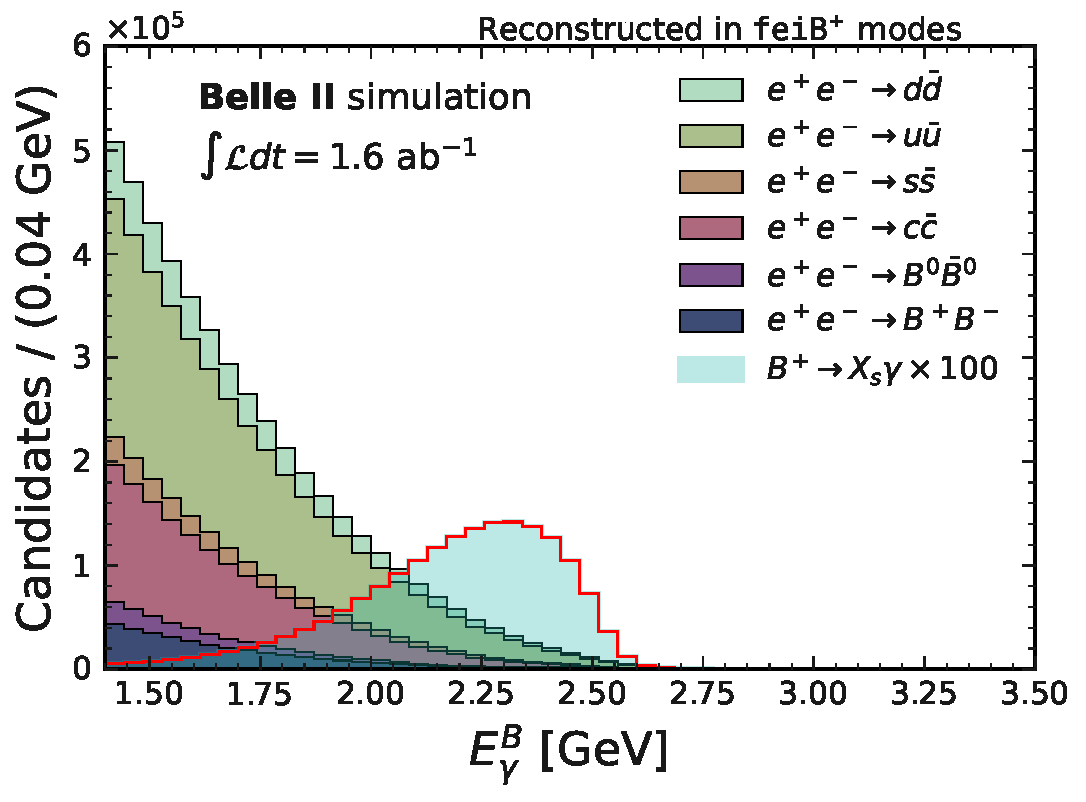
\includegraphics[width=0.395\textwidth]{figures/continuum_suppression/Bp_tagged_background_preselection.pdf}
    }
    \subcaptionbox{\label{fig:bz_preselected_photons}}{
        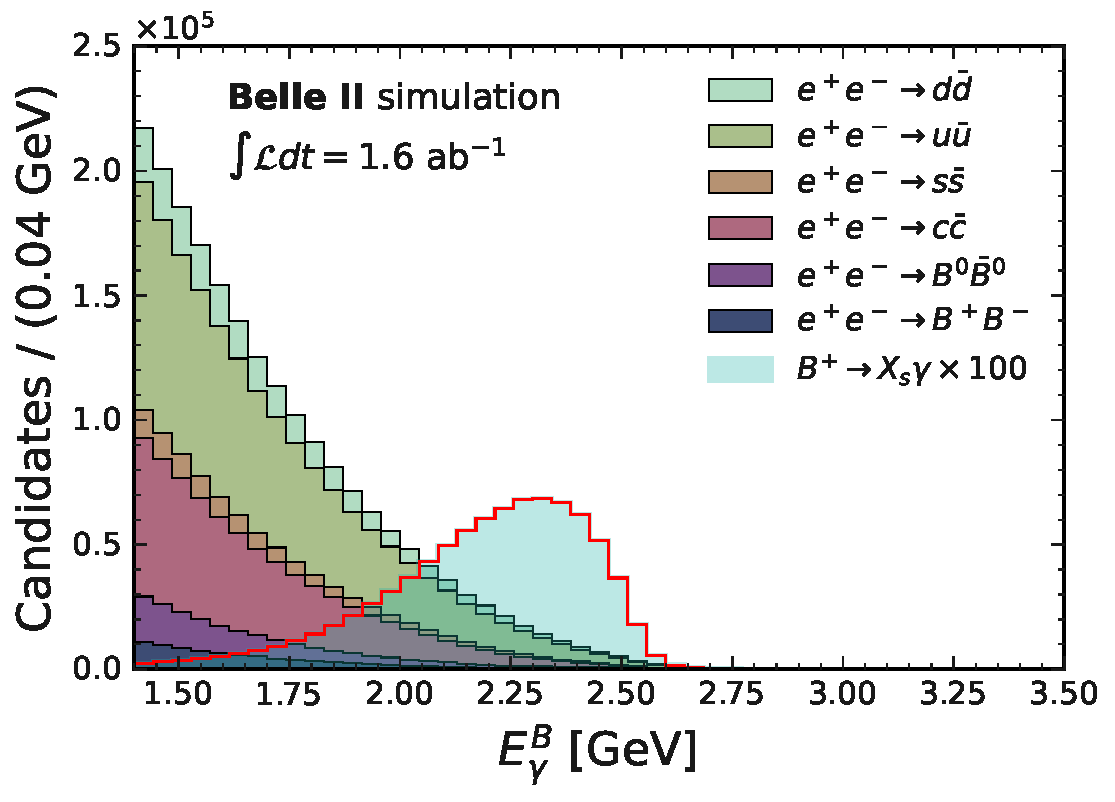
\includegraphics[width=0.395\textwidth]{figures/continuum_suppression/Bz_tagged_background_preselection.pdf}
        }
    \caption{\label{fig:preselected_photons} \BtoXsgamma spectrum in generic \MC after pre-selection for training the continuum suppression \BDT classifier.
    Overlaid are events from signal \MC where the photon comes from \BtoXsgamma, multiplied by a scaling factor.
    Compared to \Cref{fig:spectrum_after_reco}, the effectiveness of background suppression so far is apparent.
    These figures may include multiple tag entries per event.
    }
\end{figure}

Finally, many combinatorial tag-side candidates in \BB events may still contribute to the analysis at this stage.
A more detailed definition for a `well-reconstructed' tag will be explored later in \Cref{sec:good_tag_definition}.
At this stage, it is sufficient to acknowledge that the vast majority of correctly reconstructed tag-side candidates are expected to have $\Mbc>5.27~\gevcc$.
Therefore, this requirement is also adopted for optimisation studies and training in \Cref{sec:continuum_features,sec:continuum_training,sec:continuum_validation}.

\subsection{Continuum suppression feature selection}\label{sec:continuum_features}

$B$ factory experiments and Belle II have a large selection of observables that can be utilised for continuum suppression and are suitable to be input as variables to a \BDT.
These observables describe the event topology and other collective particle decay properties. 
They are optimised to provide optimal separation between \BB and \qqbar events.
Two caveats have to be kept in mind for the \BtoXsgamma analysis:
\begin{itemize}
    \item Generally, \BtoXsgamma event-topology may be different compared to \BB events. 
    \BtoXsgamma decays have a single jet-like $X_s$ system (while the other $B$ meson decays hadronically).
    This leads to a somewhat middle-case between a generic-\BB event and an \epem\ra\qqbar event, as it was illustrated in \Cref{fig:continuum_schematic}.
    \item Many of these observables contain momenta, angles or other parameters of some (or even all) particles in the event -- including the $X_s$ system and the photon.
    This may lead to a bias in the \EB spectrum.
    Furthermore, even relatively small biases over many training features may be learnt by the \BDT and introduced to the spectrum.
    \item Some features may perform differently in real data compared to simulation, due to unexpected differences in alignment, calibration or background distributions.
    As we use simulated data sets to train a \BDT in this analysis, such a comparison is crucial.
\end{itemize}
Given the mentioned points, it is important to test that observables used for the training provide adequate separation between \BtoXsgamma and \qqbar, while no bias is introduced to the photon energy spectrum.
Furthermore, this has to be well-represented in Belle~II data.

In this analysis, the following observable categories are considered for separation between \epem\ra\qqbar and \BtoXsgamma:
\begin{itemize}
    \item Various thrust-based observables (\Cref{sec:thrusts});
    \item Sphericity and aplanarity (\Cref{sec:sphericity_aplanarity});
    \item Harmonic moments (\Cref{sec:harmonic_moments});
    \item Fox-Wolfram moments (\Cref{sec:fox_wolfram_moments});
    \item Modified Fox-Wolfram moments (\Cref{sec:modified_fox_wolfram_moments});
    \item CLEO cones (\Cref{sec:cleo_cones});
    % \item Angular tag-$B$ meson observables (\Cref{sec:angular_features});
    \item Tag-$B$ meson vertex observables (\Cref{sec:vertex_features});
    \item Flavour tagger output for the tag-$B$ meson(\Cref{sec:flavour_tagger_outputs});
\end{itemize}

In total, this provides 75 potential training features that are tested to be uncorrelated to the photon energy spectrum and adequately described in simulation.
The tests use a metric of \textit{total divergence to the average} (often called \textit{Jensen-Shannon distance}) \cite{Lin:1991abc},
which is used to quantitatively evaluate the similarity between two distributions.
The Jensen-Shannon distance is bounded by 1 for two given probability distributions, $\mathbb{X}_1$ and $\mathbb{X}_2$:
\begin{equation}\label{eq:js_distance}
    0\leq\mathrm{JSD}(\mathbb{X}_1||\mathbb{X}_2) \leq1,
\end{equation}
where exactly similar distributions have a score of 0, and the score tends towards 1 when the distributions are highly-different.

Two tests are performed:
\begin{itemize}
    \item \textbf{Test 1}: $\mathbf{\EB,~\Estar~and~tag\mbox{-}side~\Mbc~bias~test}$:
    to ensure that the classifier does not indirectly select particular $X_s$ or tag-side $B$ channels,
    each tested potential training feature is separated into 5 equally populated regions (\textit{slices}) of \BtoXsgamma events in signal \MC.
    For this test, \BptoXsgamma and \BztoXsgamma are merged.
    In each of these regions, the distribution of \EB, \Estar and \Mbc is compared.
    The Jensen-Shannon distance is required to not be larger than 6\% between any two given slices of a training feature.
    The requirement to pass \textbf{Test 1} has been chosen by observing the typical values of the agreement shown by the tested unbiased distributions.
    If this requirement is not passed by at least one of the distributions (\EB, \Estar or \Mbc), the feature is excluded from the list of final \BDT training features.
    \item \textbf{Test 2}: $\mathbf{\epem\ra\qqbar~data\mbox{-}simulation~similarity~test}$:
    to ensure that simulations adequately describe the data sets that we aim to suppress.
    This test is only performed if \textbf{Test~1} is passed.
    As this is a blinded analysis, off-resonance data samples are used, which only contain \epem\ra\qqbar events.
    In this case, the Jensen-Shannon distance is calculated between 
    the area-normalised distribution of a training feature in the off-resonance data set
    and the area-normalised distribution of a training feature in \epem\ra\qqbar simulation.
    The metric is required to be no more than 10\%.
    The looser requirement is adopted here because some difference is expected between the distributions:
    the collision energy in the off-resonance data set is different to the one in the on-resonance simulation that is used in this analysis.
    Furthermore, an overall smaller off-resonance data set ($\sim19~\invfb$, see \Cref{sec:data_samples}) may have certain differences due to statistical fluctuations.
\end{itemize}

The tested distributions have the selections from \Cref{sec:preselection} included, except for the case of the off-resonance dataset, where the $\Mbc>5.27~\gevcc$ requirement is lifted.
For every event, when more than one tag-side candidate $B$ candidate exists, a random one is picked.
The application of \textbf{Test~1} with exact definitions for the 81 observables are shown in \Cref{sec:appendix_continuum_features}.

Out of 75 potential training features, 27 pass through the requirements of \textbf{Test~1}.
These are passed to \textbf{Test~2}.
Owing to the excellent calibration and simulation quality of Belle II, this requirement only removes a single feature.
The results for the 26 final observables that pass both test requirements and will be used as features in the \BDT training
are shown in \Cref{tab:passing_test1}.

\begin{table}[htbp!]
    \centering
    \caption{\label{tab:passing_test1}The training features for the \epem\ra\qqbar suppression
    that pass the requirements of \textbf{Test~1} (see \Cref{sec:appendix_continuum_features}) and \textbf{Test~2} (see \Cref{sec:appendix_continuum_features_datamc}).
    The table also shows the value of the Jensen-Shannon distances for each observable for the different requirements of both tests.
    Exact definitions of these quantities are provided in \Cref{sec:appendix_continuum_features}.
    Observable groups follow those introduced in the text.
    }   
    \begin{tabular}{l|c|c|c|c|}
    \multirow{3}{*}{Feature name} & \multicolumn{4}{|c|}{Jensen Shannon Distances [$\sqrt{\mathrm{bit}}$]}\\
                                  & \multicolumn{3}{|c|}{Test~1} & Test~2\\
                                  & \EB& \Estar& \Mbc & Data-Sim.\\
    \hline
    \multicolumn{5}{c|}{\textbf{Thrust related}}\\
    \hline
    $\cos\theta_{\mathrm{TB}\wedge\mathrm{TO}}$ & 0.03 & 0.01 & 0.04 & 0.02\\
    $\cos\theta_{\mathrm{TB}\wedge\mathrm{z}}$ & 0.01 & 0.01 & 0.02 & 0.01\\
    $T_{\mathrm{B}}$ & 0.04 & 0.03 & 0.04 & 0.06\\
    $\cos\theta_{\mathrm{T}}$ & 0.02 & 0.02 & 0.01 & 0.02\\
    \hline
    \multicolumn{5}{c|}{\textbf{Harmonic moments}}\\
    \hline
    $B_{1}^T$ & 0.05 & 0.05 & 0.02 & 0.01\\
    $B_{3}^T$ & 0.04 & 0.03 & 0.01 & 0.03\\
    \hline
    \multicolumn{5}{c|}{\textbf{CLEO cones}}\\
    \hline
    $\mathtt{CC}^B_0$ & 0.04 & 0.03 & 0.03 & 0.03\\
    $\mathtt{CC}^B_1$ & 0.03 & 0.03 & 0.02 & 0.03\\
    $\mathtt{CC}^B_2$ & 0.04 & 0.03 & 0.02 & 0.01\\
    $\mathtt{CC}^B_3$ & 0.05 & 0.05 & 0.02 & 0.02\\
    $\mathtt{CC}_0$ & 0.05 & 0.05 & 0.02 & 0.02\\
    $\mathtt{CC}_3$ & 0.06 & 0.06 & 0.02 & 0.02\\
    \hline
    \multicolumn{5}{c|}{\textbf{Modified Fox-Wolfram moments}}\\
    \hline
    $H_{c4}^{so}$ & 0.05 & 0.04 & 0.02 & 0.02\\
    $H_{m2}^{so}$ & 0.03 & 0.03 & 0.02 & 0.02\\
    $H_{m4}^{so}$ & 0.03 & 0.03 & 0.01 & 0.01\\
    $H_{0}^{oo}$ & 0.03 & 0.02 & 0.02 & 0.04\\
    \hline
    \multicolumn{5}{c|}{\textbf{Tag-$\mathbf{B}$ meson vertex observables}}\\
    \hline
    $z$ of tag-B & 0.01 & 0.01 & 0.01 & 0.02 \\
    $\Delta x$ of tag-B & 0.02 & 0.02 & 0.03 & 0.03\\
    $\Delta y$ of tag-B & 0.01 & 0.01 & 0.03 & 0.04\\
    $\Delta z$ of tag-B & 0.02 & 0.02 & 0.04 & 0.02\\
    $\Delta \tau$ & 0.04 & 0.03 & 0.02 & 0.02\\
    $\Delta z$ & 0.04 & 0.03 & 0.02 & 0.02\\
    $\Delta z_B$ & 0.04 & 0.03 & 0.02 & 0.02\\
    $\chi^2_{B_{\mathrm{ROE}};\mathrm{IP}}$ & 0.05 & 0.05 & 0.01 & 0.00\\
    $x_{B_{\mathrm{ROE}}}$ & 0.03 & 0.03 & 0.01 & 0.02\\
    $z_{B_{\mathrm{ROE}}}$ & 0.03 & 0.03 & 0.01 & 0.05\\
\end{tabular}

\end{table}

\subsection{Continuum suppression training}\label{sec:continuum_training}

As it was argued in \Cref{sec:continuum_features}, events containing \BtoXsgamma decays may have slightly different kinematic properties compared to a generic-\BB.
Although these differences, as seen in \Cref{sec:appendix_continuum_features_datamc} are not large, training a classifier to separate generic $\FourS\ra\BB$ and \epem\ra\qqbar events may lead to a suboptimal separation of \BtoXsgamma.

A more effective setup is to remove \BB events from generic \MC and supplement the leftover events with \BtoXsgamma events from signal \MC. 
In such a scenario, the classifier learns to distinguish between the signal decays and continuum events, without the additional ambiguity of including generic \BB decays.
All selections from \Cref{tab:preselections} are employed for the training datasets.

The training samples are prepared by creating a mixture of $100000$ \epem\ra\qqbar events and 100000 \BtoXsgamma events from the signal MC sample.
In each event, one $\gamma$ and $\B_{\mathrm{tag}}$ candidate combination is randomly chosen.
This requirement ensures that the same event cannot contribute multiple training entries.
The target variable for the training is defined as a $\mathtt{flag}$, which follows
\begin{equation}
    \mathtt{flag}=\begin{cases}
      0,\quad \mathrm{for}~\epem\ra\qqbar~\mathrm{events},\\ 
      1,\quad \mathrm{for}~\BtoXsgamma~\mathrm{events}.
      \end{cases}
\end{equation}
Half of the \epem\ra\qqbar training sample is taken from the \feiBp mode, and the other half is from \feiBz modes. 
For signal, half is taken from $\BptoXsgamma$ signal mode, the other half from $B^0$, irrespective of the \FEI mode.
An equivalent sample is prepared as the testing sample for the training.

The training is performed using a \texttt{FastBDT} algorithm, introduced in \Cref{sec:BDTs_theory}.
Four hyperparameters within \texttt{FastBDT} framework have to be chosen.
Hyperparameter optimisation is performed in a grid-like search, based on two quantities:
\begin{align}\label{eq:optimisation_criteria}
    \begin{split}
    \mathtt{AUC}_{\mathrm{test}}&;\\
    \Delta \mathtt{AUC} \equiv |\mathtt{AUC}_{\mathrm{train}}& - \mathtt{AUC}_{\mathrm{test}}|,\\
    \end{split}
\end{align}
where $\mathtt{AUC}_{\mathrm{train}/\mathrm{test}}$ is the \AUC score for training or testing samples.
A set of hyperparameters is sought, such that $ \mathtt{AUC}_{\mathrm{test}}$ is maximised, while $\Delta \mathtt{AUC}$ is minimised.
The results of hyperparameter optimisation are summarised in \Cref{tab:grid_search} and shown in \Cref{fig:hyper_param}
Larger depth or number of trees are not explored to avoid non-linear correlations which may be learnt by the classifier and would require additional studies to pinpoint.
Large shrinkage values are undesired, to ensure a slower learning rate of the classifier.

\begin{table}[htbp!]
    \centering
    \caption{\label{tab:grid_search}Hyperparameter optimisation based on a grid-search method.
    The four hyperparameters for the \texttt{FastBDT} algorithm are defined in \Cref{sec:BDTs_theory}.
    The optimal values are chosen based on criteria defined in \Cref{eq:optimisation_criteria}.
    They are shown in the rightmost column and taken as the parameters for the training.
    The corresponding $\mathtt{AUC}_{\mathrm{test}}$ and $\Delta \mathtt{AUC}$ are shown in \Cref{fig:hyper_param} and \Cref{fig:roc_curve}.
    }
    \begin{tabular}{l|c|c|}
    Hyperparameter     & Tested grid values       & Chosen optimal parameter \\
    \hline 
    depth              & \{1,2,3\}                  & 2    \\
    number of trees    & \{100,200,400,600,1000\} & 400  \\
    shrinkage          & \{0.01,0.05,0.1,0.3,0.5\}          & 0.1  \\
    training subsample & \{0.2,0.4,0.5,0.6,0.8\}  & 0.8  \\
\end{tabular}

\end{table}

\begin{figure}[htbp!]
    \centering
    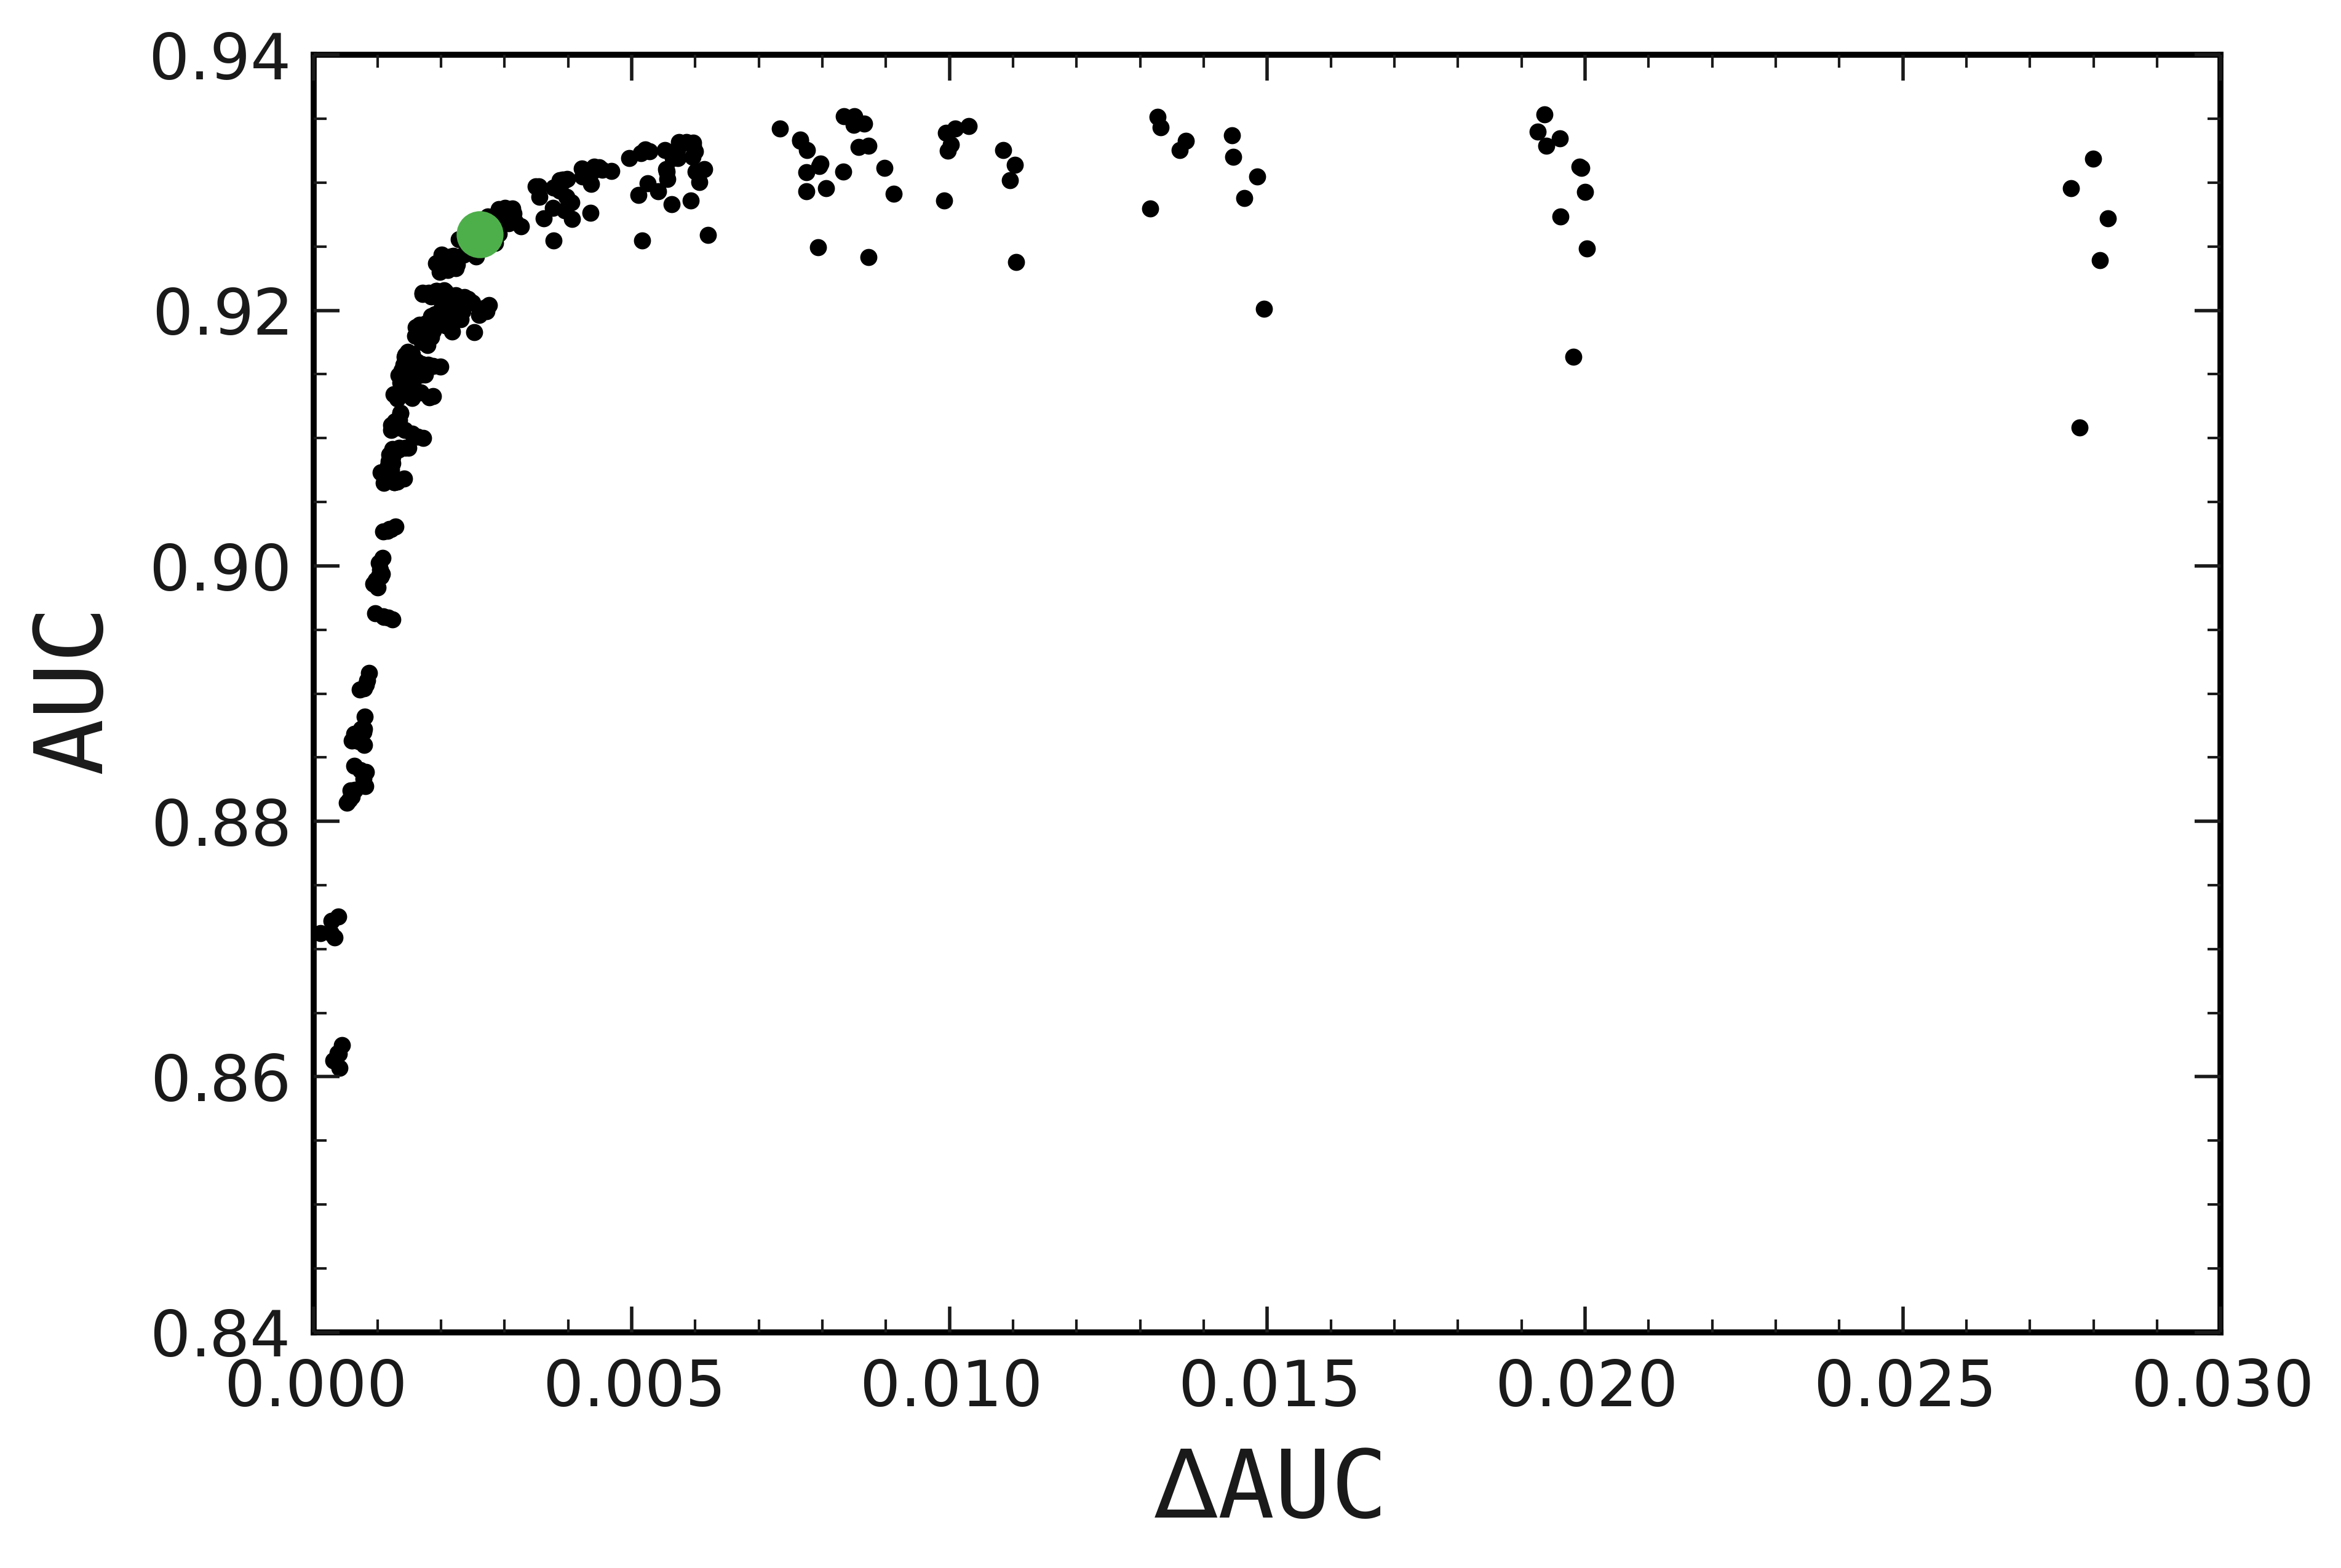
\includegraphics[width=0.45\textwidth]{figures/continuum_suppression/hyperpar_optimisation.png}
    \caption{\label{fig:hyper_param}Hyperparameter optimisation as a function of quantities defined in \Cref{eq:optimisation_criteria}.
    In total 375 working points are tested.
    The choice of parameters, shown in \Cref{tab:grid_search}, is represented by the enlargened green point.
    It is chosen in the threshold area, where $\mathtt{AUC}_{\mathrm{test}}$ gain saturates and $\Delta \mathtt{AUC}$ gain accelerates.
    }
\end{figure}

The training is performed with features from \Cref{tab:passing_test1} and hyperparameters from \Cref{tab:grid_search}.
The normalised classifier output for test and train samples is shown in \Cref{fig:separation_curve}.
It is seen that the classifier shows almost no bias, as the train and test samples agree very well.
This is further alluded to by inspecting the ROC curve in \Cref{fig:roc_curve}.
Inspecting the ROC curves no significant differences are observed.
The difference in the \AUC scores is smaller than 1\%.
\begin{figure}[htbp!]
    \centering
    \subcaptionbox{\label{fig:separation_curve}}{
    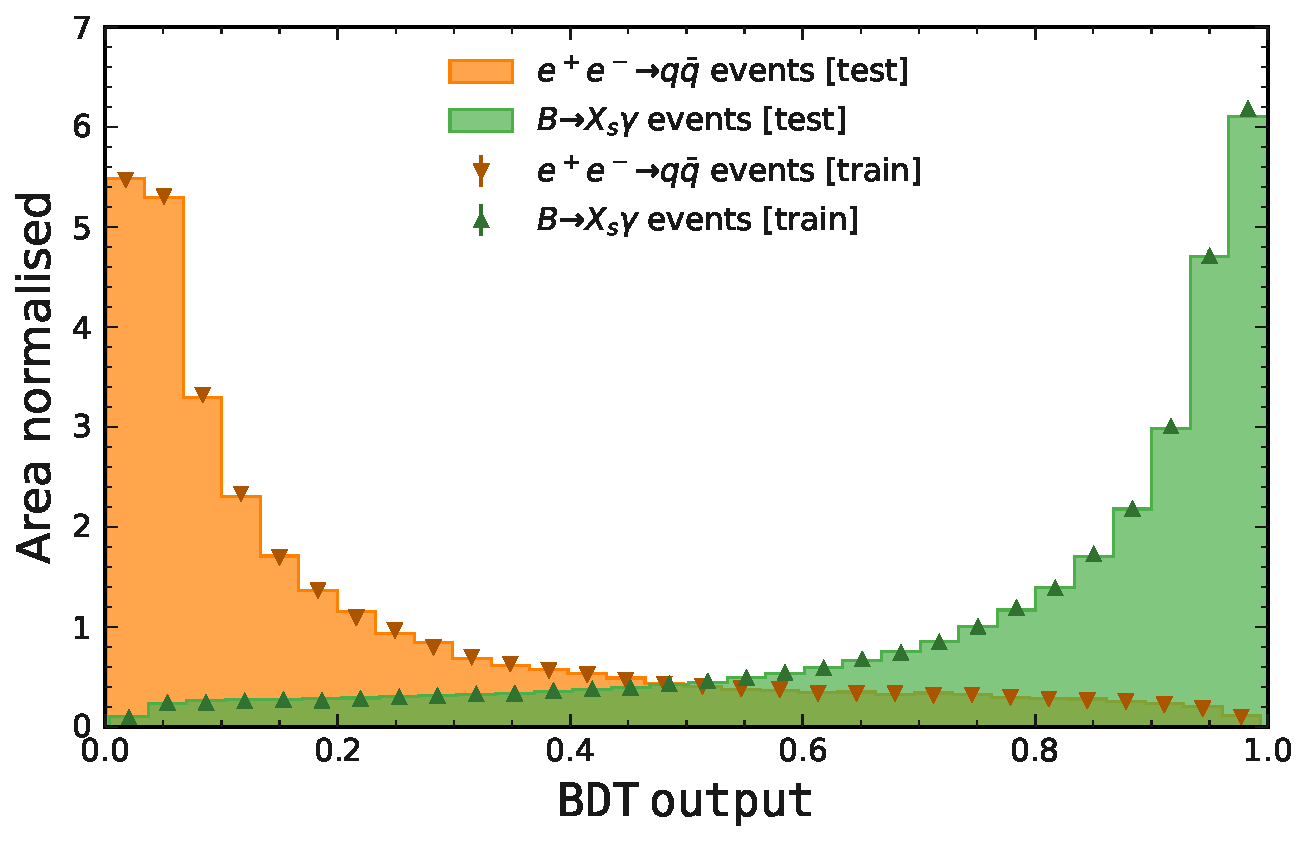
\includegraphics[width=0.45\textwidth]{figures/continuum_suppression/separation_curves.pdf}
    }
    \subcaptionbox{\label{fig:roc_curve}}{
        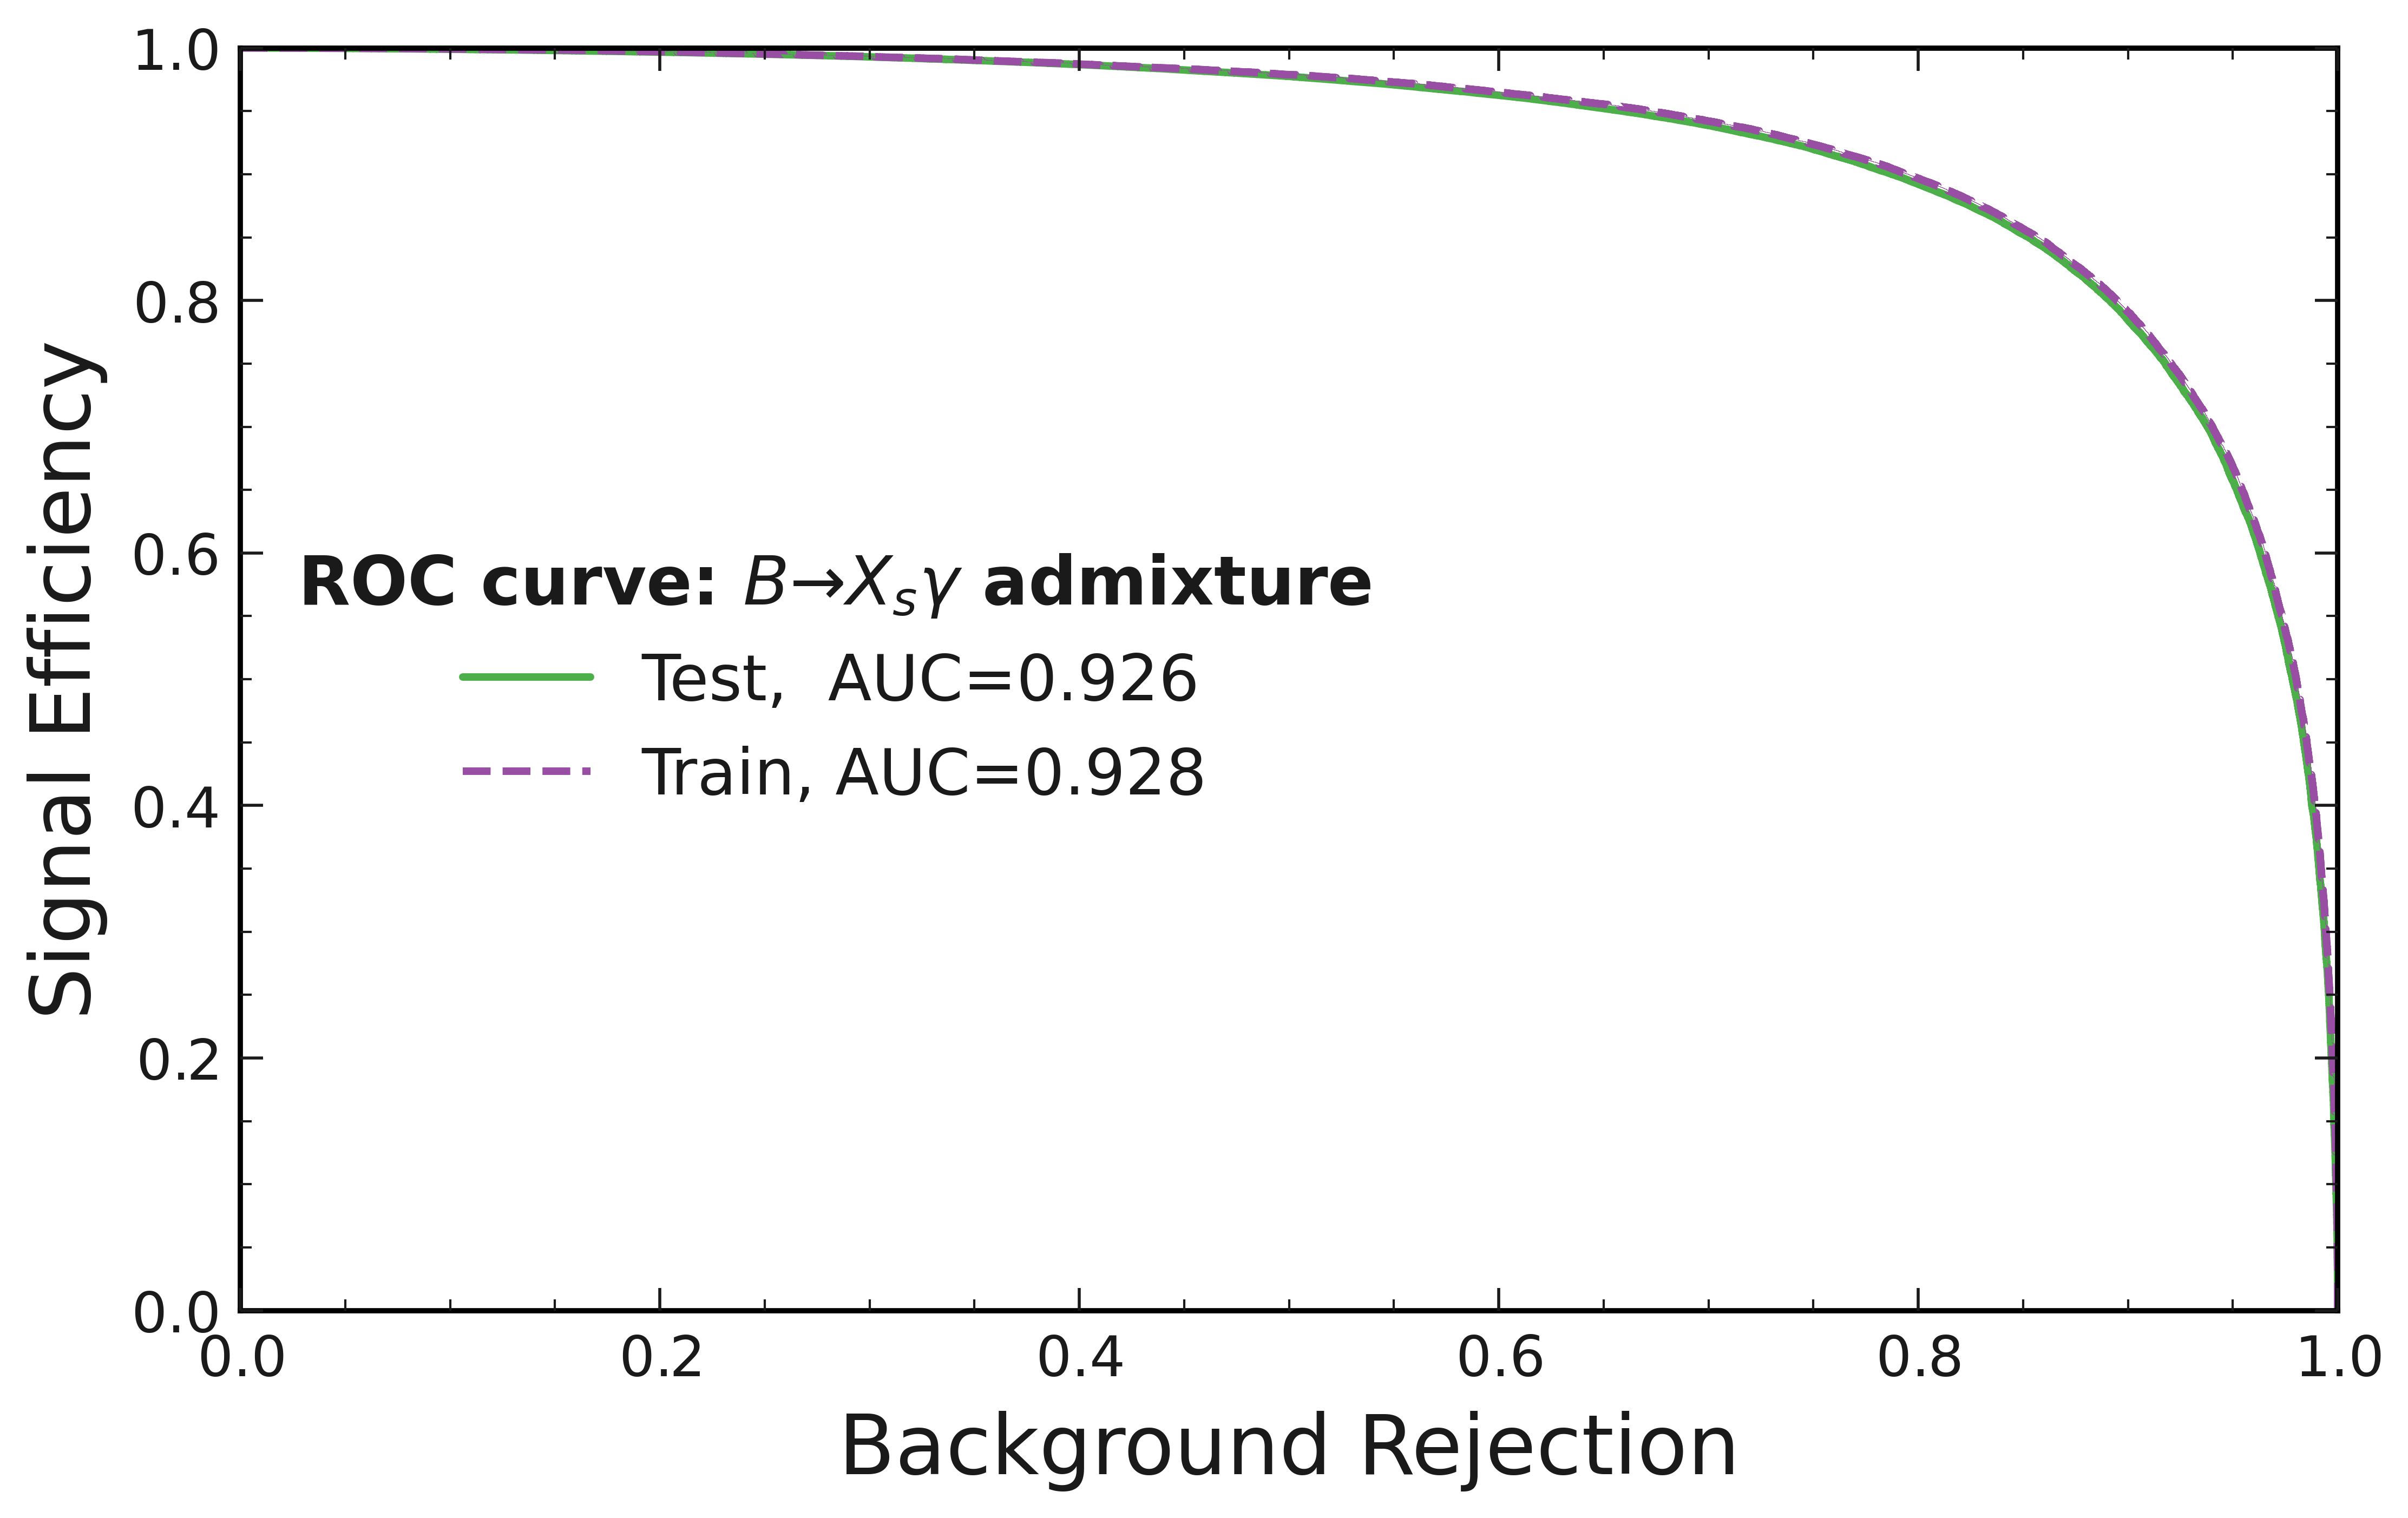
\includegraphics[width=0.45\textwidth]{figures/continuum_suppression/roc_curve.png}
    }
    \caption{\label{fig:training_evaluation} The training evaluation for this analysis.
    \Cref{fig:separation_curve} shows excellent separation between \epem\ra\qqbar and \BtoXsgamma samples and excellent agreement between corresponding test and train samples.
    \Cref{fig:roc_curve} shows the \ROC curve of the training. 
    The test and train sample \AUC scores are close to unity and similar, alluding to a high-separation power that is observed, and no evidence of overtraining.
    }
\end{figure}

Using the tools provided by the \texttt{FastBDT} algorithm, a \textit{relative feature importance} is computed.
Particularly for \texttt{FastBDT}, it is computed by evaluating the decrease of the \AUC score if the feature is not included in the training dataset (for more details see Ref.\cite{Keck:2017gsv}.)
Therefore, it can be considered a quantitative measure of the impact of a feature on the final classifier output.
The figure depicting relative training observable importance is shown in \Cref{fig:feature_importance}. 
It is seen that $\cos\theta_{\mathrm{TB}\wedge\mathrm{TO}}$ -- angle between the thrust axis of the tag-$B$ candidate and everything else in the event. 
-- has by far the largest impact on the classifier.
This is not surprising after inspecting the individual separation power for the current problem in \Cref{sec:appendix_continuum_features_datamc}.
Other important separation features come from  $\Delta z_B$ \&  $\Delta z_B$, related to the longitudinal distance between the decay vertices,
thrust of the tag-$B$ meson, $T_B$ and CLEO cone variables $\mathtt{CC}_i$. 
For consistency, the events used in the training are removed from further analysis, although their impact is negligible.

\begin{figure}[htbp!]
    \centering
    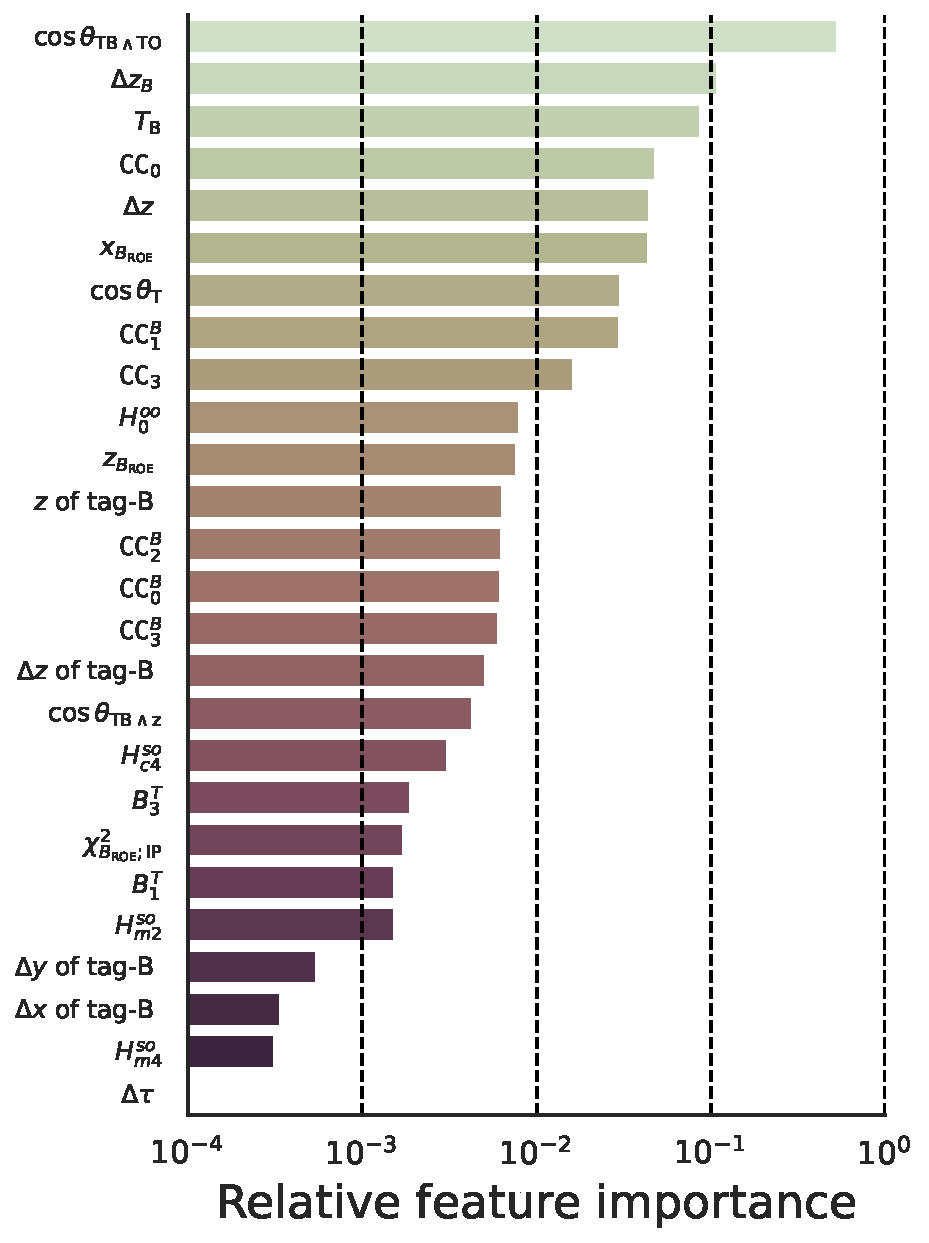
\includegraphics[width=0.45\textwidth]{figures/continuum_suppression/feature_importance.pdf}
    \caption{\label{fig:feature_importance} The relative feature importances of different observables used in the training.
    The definitions of these observables are provided in \Cref{sec:appendix_continuum_features}.
    The feature importance highlights a relative change in \AUC score when the observable is not included in the training.
    }
\end{figure}

\subsection{Continuum suppression validation}\label{sec:continuum_validation}

The resulting $\mathtt{BDT~output}$ is tested photon energy spectrum to further ensure the validity of the training.
Following the tests for bias of the average, median and $1\sigma$ percentiles in \Cref{sec:signal_photon_correlation},
the same study is performed for the training classifier output.
The result is shown in \Cref{fig:bdt_output_correlation} for the \BtoXsgamma admixture sample with the same requirements as the training sample.
No significant bias to any of the photon-energy spectrum quantities is observed in any of the intervals.
In \Cref{fig:bdt_data_shape} the trained classifier output is also applied to the off-resonance data.
Comparing the shapes of off-resonance data and simulation adequate agreement is observed, particularly in the high-$\mathtt{BDT~output}$ region where most signal lies.
The results seen in \Cref{fig:bdt_validation} validate the fact that the \BDT is prepared in an unbiased way and strongly suppresses the continuum events.
\begin{figure}[htbp!]
    \centering
    \subcaptionbox{\label{fig:bdt_output_correlation}}{
    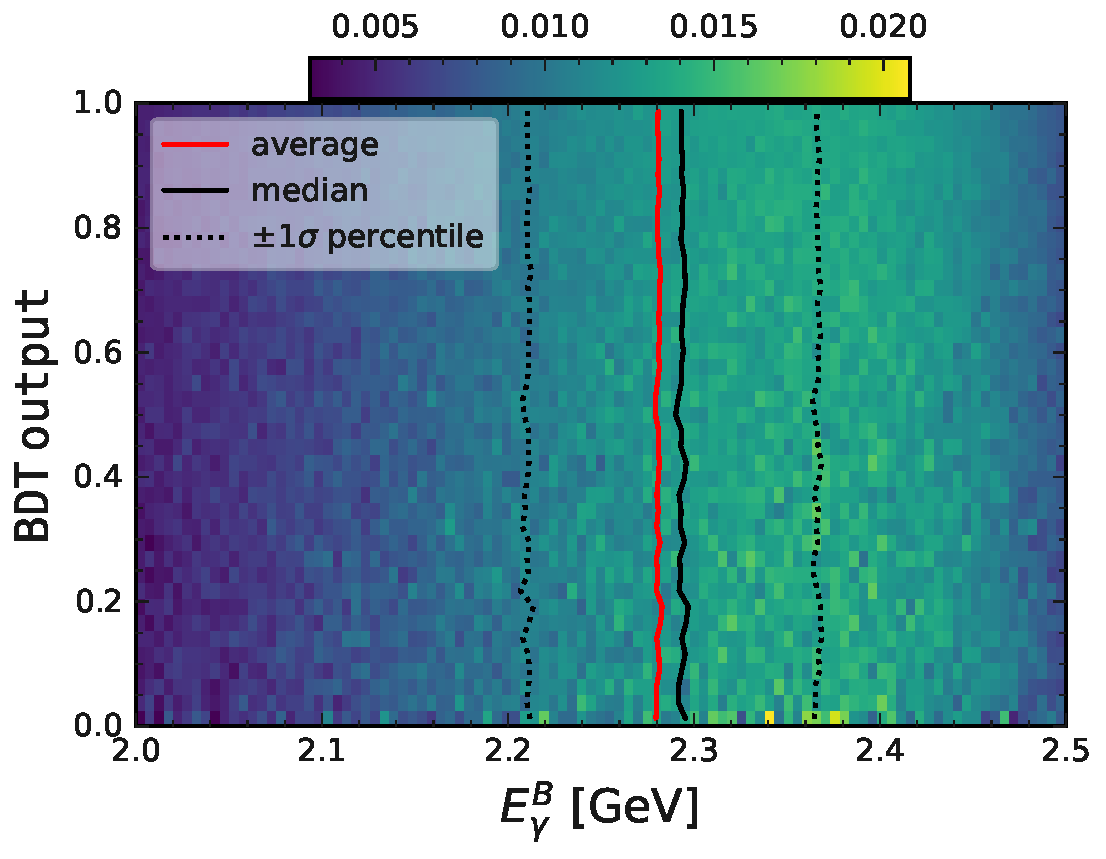
\includegraphics[width=0.4\textwidth]{figures/continuum_suppression/BDT_output_correlation.pdf}
    }
    \subcaptionbox{\label{fig:bdt_data_shape}}{
        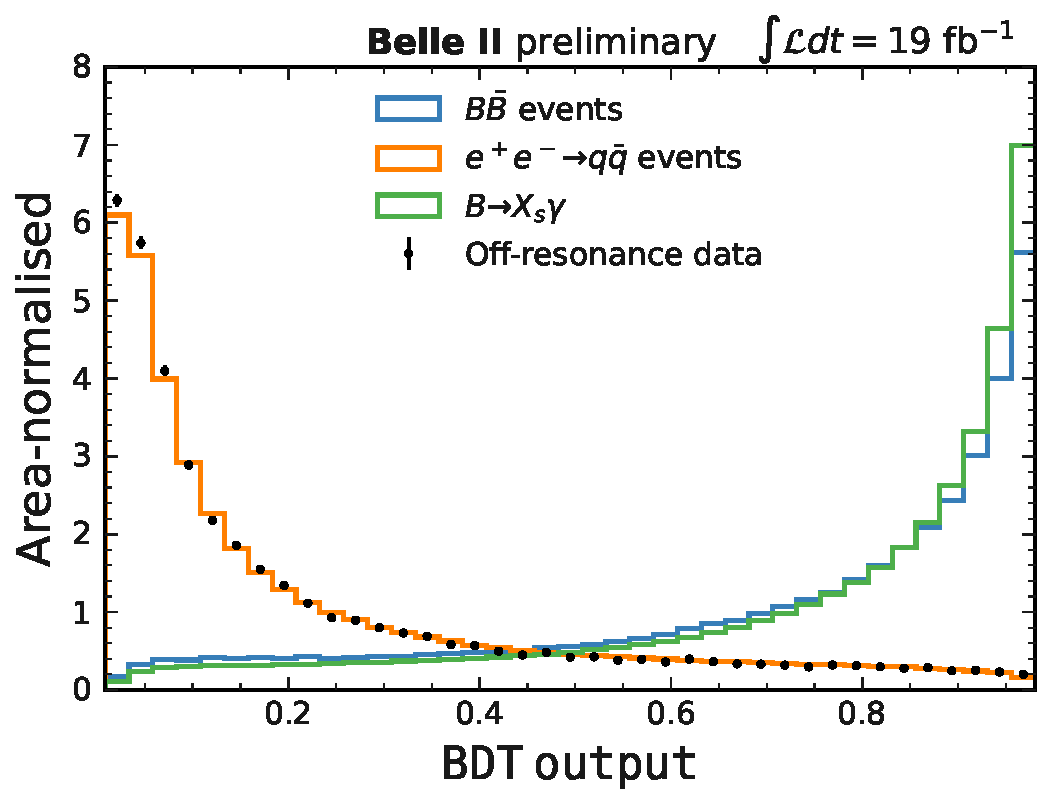
\includegraphics[width=0.4\textwidth]{figures/continuum_suppression/trained_bdtBDT_output_test.pdf}
        }
    \caption{\label{fig:bdt_validation} 
    Validation of the training described in \Cref{sec:continuum_training}.
    In \Cref{fig:bdt_output_correlation}, correlation tests for the trained classifier output described in \Cref{sec:continuum_training}, depicted as a 2D histogram.
    Each row is normalised, such that all bins within that row add up to 1.
    In the red line, the average photon energy, $\expval{\EB}$, is shown as a function of the tested observable.
    In black and black-dotted lines -- median and $\pm 1 \sigma$ percentile values of \EB, respectively.
    No strong dependence can be observed in any of the quantities or the 2D maps.
    In \Cref{fig:bdt_data_shape}, the shape of \epem\ra\qqbar and off-resonance data is compared.
    It is seen that both simulated and off-resonance data sets are well separated from \BB and \BtoXsgamma simulation.
    }
\end{figure}